% !TEX root = DesignDocument.tex

\chapter{User Stories,  Requirements, and Product Backlog}
\section{Overview}

This section contains the features, creation, and develpment of crowd control. It covers prerequsite user stories, to the design and implimentation of the application its self.

%The overview should take the form of an executive summary.  Give the reader a feel 
%for the purpose of the document, what is contained in the document, and an idea 
%of the purpose for the system or product. 

 %The user stories 
%are provided by the stakeholders.  You will create he backlogs and the requirements, and document here.  
%This chapter should contain 
%details about each of the requirements and how the requirements are or will be 
%satisfied in the design and implementation of the system.

%Below:   list, describe, and define the requirements in this chapter.  
%There could be any number of sub-sections to help provide the necessary level of 
%detail. 




\section{User Stories}

\subsection{User Story \#1 }
As a user I want to join a public group.

\subsubsection{User Story \#1 Breakdown}
The user can request to join any public group.  Their request will be sent to the group leader for approval.  Depending on the group leaders action then the user will be accepted or denied access to the group. 

\subsection{User Story \#2 }
As a user i want to be able to join a private group.

\subsubsection{User Story \#2 Breakdown}
For the user to join a private group they must first recieve an invitation from the group leader of the private group of interest.  Then the user can either accept or reject the invitation to join the group.  If the invitation is accepted then the user is placed into the group and then starts sharing information. 

\subsection{User Story \#3} 
As a user i want to see where the other members of my group are on a map

\subsubsection{User Story \#3 Breakdown}
Once the user is in a group then the user will have access to a map that displays markers representing the locations of all users that are members of the group.

\subsection{User Story \#4} 
As a user i want to see a list of public groups nearby

\subsubsection{User Story \#4 Breakdown}
For a user to have quick access to groups nearby that have been listed as public, once the user has logged in a list of public groups near the users current location will be displayed.

\subsection{User Story \#5} 
As a user i want to have suggestions of local activities and locations.

\subsubsection{User Story \#5 Breakdown}
Once the user joins a group there will be a tab that lists possible locations and activities nearby the user.  These suggestions will be generated by local events and businesses that advertise with Crowd Control.

\subsection{User Story \#6} 
As a user i want to leave a group.

\subsubsection{User Story \#6}
Much like joining a group the user would like to leave a group at any time and this process to be as painless as possible.  Using a button on the main group page will allow a user to leave the current group for whatever their reason.

\subsection{User Story \#7} 
As a user I want the abilitiy to login with a custom account.

\subsubsection{User Story \#7 Breakdown}
For a user to be registered with our system they will have to login.  This gives the option for the user to login with a custom Bowtaps login.

\subsection{User Story \#8}
As a user I want to login with Facebook

\subsubsection{User Story \#8 Breakdown}
If the user does not want to create a custom Bowtaps login to have access to our app,  then they can login with their facebook account.  This gives the user easy access to the app and deals with authentication with facebook.

\subsection{User Story \#9}
As a user I want to login with Twitter
\subsubsection{User Story \#9 Breakdown}
If the user does not want to create a custom Bowtaps login to have access to our app, then they can login with their Twitter account.  This gives the user easy access to the app and authentication takes place with Twitter.
\subsection{User Story \#10}
As a user I would like to message other members of the group.
\subsubsection{User Story \#10}
To keep users within our app rather than having to use another app to send a message to the group, the user can access the message tab once inside a group.  Then the user can send a single message to each member of the group.

\subsection{User Story \#10} 
As a user i would like my information protected.
\subsubsection{User Story \#10 Breakdown}
To users data protection is a major concern.  In the app all of the communication is done with user data protection in mind.  All of the data being passed back and forth between users will be sent using encrypted strings. 

\subsection{User Story \#11} 
As a group leader I want to be able to create an Itinerary for the group
\subsubsection{User Story \#11 Breakdown}
The group leader can create an Itinerary for all group members to be able to view.  This can contain waypoints or just times when special events in the group will occur.

\subsection{User Story \#12}
As a user I want to be able to look at my groups itinerary.
\subsubsection{User Story \#12 Breakdown}
If the group leader has created an itinerary for the group the users would like access to see upcoming group events and locations.

\subsection{User Story \#13}
As a group leader I would like to invite members to a private group
\subsubsection{User Story \#13 Breakdown}
To join a private group the group leader must send an invitation to the members that would like to join. 

\section{Requirements and Design Constraints}
%Use this section to discuss what requirements exist that deal with meeting the 
%business need.  These requirements might equate to design constraints which can 
%take the form of system, network, and/or user constraints.  Examples:  Windows 
%Server only, iOS only, slow network constraints, or no offline, local storage capabilities. 

This section contains the requirements and constraints of all aspects of Crowd Control.  This includes requirements and constraints for both iOS and Android operating systems, server side, and network.


\subsection{System Requirements}

Crowd Control is being developed to run on two different mobile operating systems, iOS and Android.  Although both applications will adhear to the same user stories, some requirements and implementation details differ.  Below each operating system is outlined with its specific requirements.

\subsubsection{iOS Requirements}
\begin{itemize}
\item{Use Apple Mapping Features}
\item{Connect with Parse API for backend data storage}
\end{itemize}
\subsubsection{Android Requirements}
\begin{itemize}
\item{Use Google Maps}
\item{Connect with Parse API for backend data storage}
\end{itemize}
\subsubsection{Parse Requirements}
\begin{itemize}
\item{Add users to groups}
\item{Remove users from groups}
\end{itemize}

\subsection{Network Requirements}

Network requrements are mobile networks as this is a mobile applications. The requirement on our part is making sure that the application is able to reach the server and use at little data as possible when connected to the network. Making sure we use as little data as possible will help our users not use all of their data. 

\subsection{Development Environment Requirements}
%What are they?  Is the system supposed to be cross-platform?
To develop Crowd Control natively for Android and iOS, two different IDEs will be used.  For iOS, development must be done on an Apple device.  The IDE used is XCode which has all of the necessary SDKs and emulation software to develop and test the iOS version of Crowd Control.  For Android, development happens on the Android Studio IDE which like Apple's XCode, also contains the necessary development tools required to develop for Android.  Android Studio can be run on either  Windows and Mac. 

\subsection{Project  Management Methodology}
%The stakeholders might restrict how the project implementation will be managed. 
 %There may be constraints on when design meetings will take place.  There might 
%be restrictions on how often progress reports need to be provided and to whom. 

We have set restrictions on the developemnt of Crowd Control and are listed as follows:
 
\begin{itemize}
\item GitHub issues will be used to keep track of current status as well as backlogs for the product.
\item There will be 3 total sprints over 2 semesters for this products.
\item The sprint cycles are 3 weeks long.
\item Progress reports will be summited to Dr. McGough and Brian Butterfeild at the end of each sprint.
\item 4 Github repositories will be used for source control, one for each platform, one for the server code, and one for documentation. 
\end{itemize}


\section{Specifications}  
Crowd Control is to be built for the two largest mobile operating systems, Android and iOS.  This choice was made to support the two most used smartphone operating systems because between these two, they support 94.7\% of the smartphone market.  Also considering the time restriction of full-time students and the length of Senior Design, the main operating system for development will be Android.

\section{Product Backlog}
%The full product backlog should go here.  The sprint backlogs are located in the project chapter.

 
\begin{itemize}
\item What system will be used to keep track of the backlogs and sprint status?
\item Will all parties have access to the Sprint and Product Backlogs?
\item How many Sprints will encompass this particular project?
\item How long are the Sprint Cycles?
\item Are there restrictions on source control? 
\end{itemize}


\section{Research or Proof of Concept Results}
%This section is reserved for the discussion centered on any research that needed 
%to take place before full system design.  The research efforts may have led to 
%the need to actually provide a proof of concept for approval by the stakeholders. 
 %The proof of concept might even go to the extent of a user interface design or 
%mockups. 


The Proof of concept is a rough design that implements basic features of Crowd Control. Basic features are currently under construction. This is currently a functional prototype with improvements in the future.
\newline 
\newline
Below are screen shots of both android and iOS proof of concepts.
(current formatting issues need to fix)
\subsection{iOS Proof of Concept Screen Shots}

Below are screen shots from the iOS version of Crowd Control.


	\begin{figure}[!tbh]
	\begin{center}
	\fbox{\includegraphics[scale=.1 ]{Additional/iOS/iOSPictures/img_3901.png}}
	\end{center}
	\caption{iOS login select screen \label{iOSloginselectscreen}}
	\end{figure}

	\begin{figure}[!tbh]
	\begin{center}
	\fbox{\includegraphics[scale=.1]{Additional/iOS/iOSPictures/img_3896.png}}
	\end{center}
	\caption{iOS email login screen \label{iOSemailLoginScreen}}
	\end{figure}

	\begin{figure}[!tbh]
	\begin{center}
	\fbox{\includegraphics[scale=.1]{Additional/iOS/iOSPictures/img_3897.png}}
	\end{center}
	\caption{iOS create account screen \label{iOScreateAccountScreen}}
	\end{figure}

	\begin{figure}[tbh]
	\begin{center}
	\fbox{\includegraphics[scale=.1]{Additional/iOS/iOSPictures/img_3898.png}}
	\end{center}
	\caption{iOS group infomation screen \label{iOSGroupScreen}}
	\end{figure}

	\begin{figure}[tbh]
	\begin{center}
	\fbox{\includegraphics[scale=.2]{Additional/iOS/iOSPictures/img_3899.png}}
	\end{center}
	\caption{iOS map view screen \label{iOSmapScreen}}
	\end{figure}

	\begin{figure}[tbh]
	\begin{center}
	\fbox{\includegraphics[scale=.1]{Additional/iOS/iOSPictures/img_3900.png}}
	\end{center}
	\caption{iOS messaging main screen \label{iOSmessagingMain}}
	\end{figure}


\subsection{Android  Proof of Concept Screen Shots}

Below are screen shots from the Android version of CrowdControl.


	\begin{figure}[tbh]
	\begin{center}
	\fbox{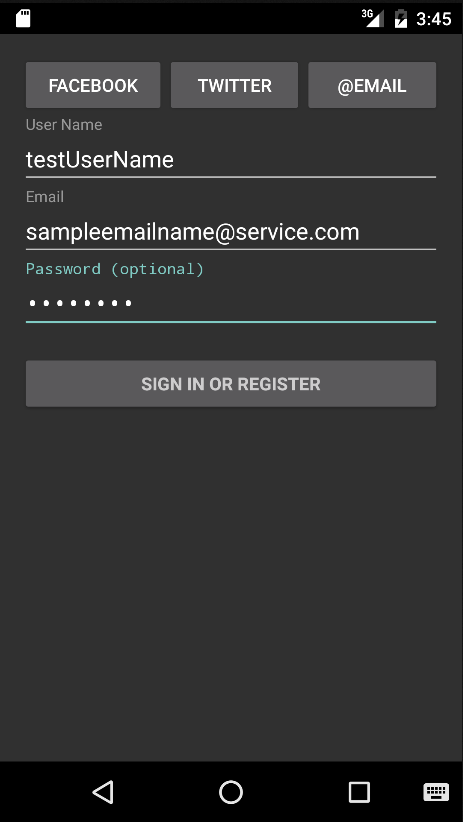
\includegraphics[scale=.4]{Additional/Android/AndroidPictures/loginScreen.png}}
	\end{center}
	\caption{Android login screen \label{AndroudLoginScreen}}
	\end{figure}

	\begin{figure}[tbh]
	\begin{center}
	\fbox{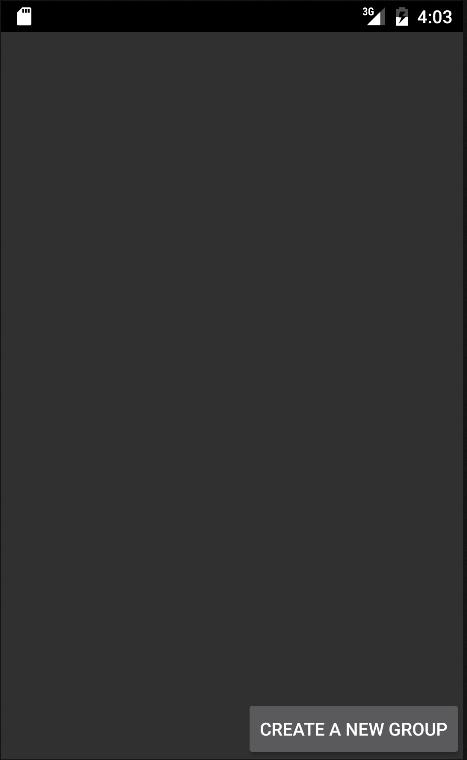
\includegraphics[scale=.4]{Additional/Android/AndroidPictures/createNewGroup.png}}
	\end{center}
	\caption{Android create group screen \label{AndroidCreateGroup}}
	\end{figure}

	\begin{figure}[tbh]
	\begin{center}
	\fbox{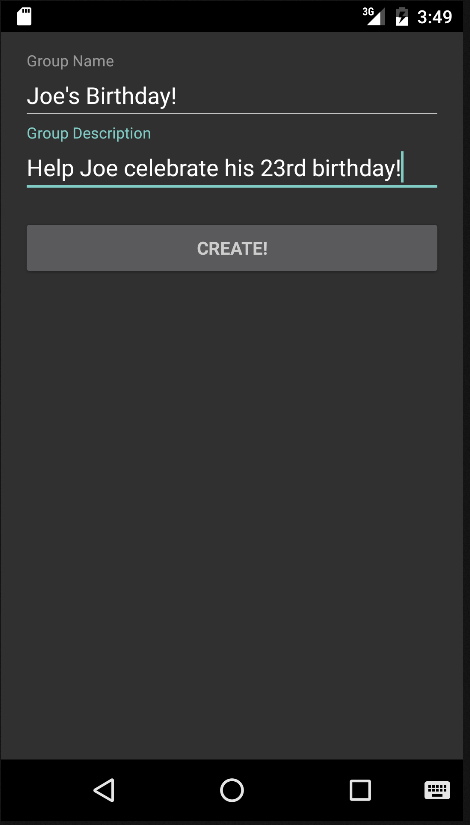
\includegraphics[scale=.4]{Additional/Android/AndroidPictures/groupCreatePage.png}}
	\end{center}
	\caption{Android group information screen \label{AndroidGroupInfo}}
	\end{figure}

	\begin{figure}[tbh]
	\begin{center}
	\fbox{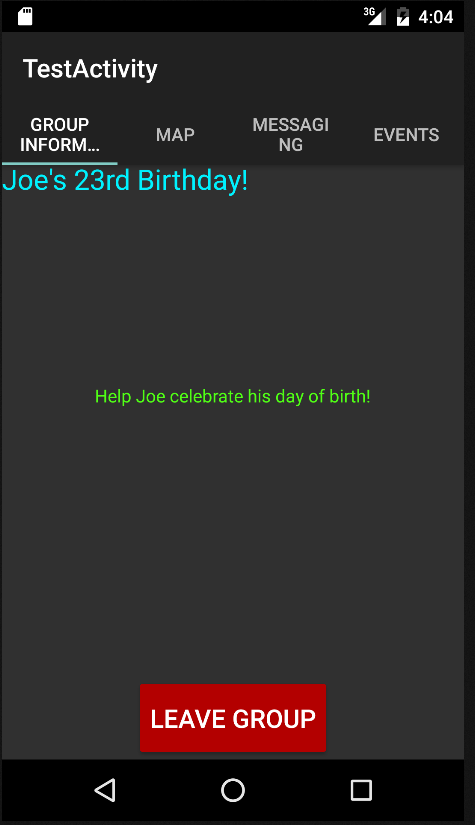
\includegraphics[scale=.4]{Additional/Android/AndroidPictures/groupJoinedPage.png}}
	\end{center}
	\caption{Android group join screen \label{AndroidJoinGroup}}
	\end{figure}

	\begin{figure}[tbh]
	\begin{center}
	\fbox{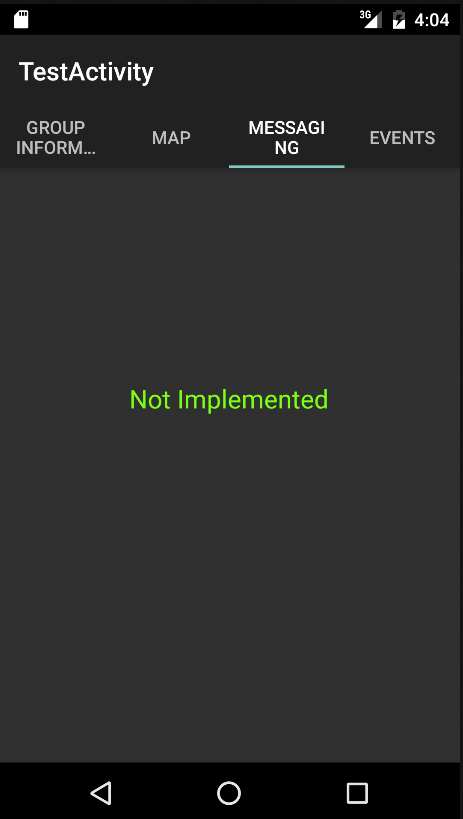
\includegraphics[scale=.4]{Additional/Android/AndroidPictures/messagingNotImplemented.png}}
	\end{center}
	\caption{Android messaging main screen \label{AndroidMessagingMain}}
	\end{figure}


\section{Supporting Material}


%This document might contain references or supporting material which should be documented 
%and discussed  either here if appropriate or more often in the appendices at the end.  This material may have been provided by the stakeholders  
%or it may be material garnered from research tasks.

